% LaTeX path to the root directory of the current project, from the directory in which this file resides
% and path to econtexPaths which defines the rest of the paths like \FigDir
\providecommand{\econtexRoot}{}\renewcommand{\econtexRoot}{.}
\providecommand{\econtexPaths}{}\renewcommand{\econtexPaths}{\econtexRoot/Resources/econtexPaths}
% The \commands below are required to allow sharing of the same base code via Github between TeXLive on a local machine and Overleaf (which is a proxy for "a standard distribution of LaTeX").  This is an ugly solution to the requirement that custom LaTeX packages be accessible, and that Overleaf seems to ignore symbolic links (even if they are relative links to valid locations)
\providecommand{\econtex}{\econtexRoot/Resources/texmf-local/tex/latex/econtex}
\providecommand{\econtexSetup}{\econtexRoot/Resources/texmf-local/tex/latex/econtexSetup}
\providecommand{\econtexShortcuts}{\econtexRoot/Resources/texmf-local/tex/latex/econtexShortcuts}
\providecommand{\econtexBibMake}{\econtexRoot/Resources/texmf-local/tex/latex/econtexBibMake}
\providecommand{\econtexBibStyle}{\econtexRoot/Resources/texmf-local/bibtex/bst/econtex}
\providecommand{\econtexBib}{economics}
\providecommand{\notes}{\econtexRoot/Resources/texmf-local/tex/latex/handout}
\providecommand{\handoutSetup}{\econtexRoot/Resources/texmf-local/tex/latex/handoutSetup}
\providecommand{\handoutShortcuts}{\econtexRoot/Resources/texmf-local/tex/latex/handoutShortcuts}
\providecommand{\handoutBibMake}{\econtexRoot/Resources/texmf-local/tex/latex/handoutBibMake}
\providecommand{\handoutBibStyle}{\econtexRoot/Resources/texmf-local/bibtex/bst/handout}

\providecommand{\FigDir}{\econtexRoot/Figures}
\providecommand{\CodeDir}{\econtexRoot/Code}
\providecommand{\DataDir}{\econtexRoot/Data}
\providecommand{\SlideDir}{\econtexRoot/Slides}
\providecommand{\TableDir}{\econtexRoot/Tables}
\providecommand{\ApndxDir}{\econtexRoot/Appendices}

\providecommand{\ResourcesDir}{\econtexRoot/Resources}
\ifnum\pdfshellescape=1
\providecommand{\rootFromOut}{..} % Path back to root directory from output-directory
\providecommand{\LaTeXGenerated}{\econtexRoot/LaTeX} % Put generated files in subdirectory
\providecommand{\EqDir}{\econtexRoot/Equations} % Put generated files in subdirectory
\else
\providecommand{\rootFromOut}{.} % Path back to root directory 
\providecommand{\LaTeXGenerated}{\econtexRoot/} % Put generated files in main directory (because not allowed in subdirectory)
\providecommand{\EqDir}{\econtexRoot/} % Put generated files in main directory
\fi
\providecommand{\econtexPaths}{\econtexRoot/Resources/econtexPaths}
\providecommand{\LaTeXInputs}{\econtexRoot/Resources/LaTeXInputs}

\documentclass[\econtexRoot/BufferStockTheory]{subfiles}
% LaTeX path to the root directory of the current project, from the directory in which this file resides
% and path to econtexPaths which defines the rest of the paths like \FigDir
\providecommand{\econtexRoot}{}\renewcommand{\econtexRoot}{.}
\providecommand{\econtexPaths}{}\renewcommand{\econtexPaths}{\econtexRoot/Resources/econtexPaths}
% The \commands below are required to allow sharing of the same base code via Github between TeXLive on a local machine and Overleaf (which is a proxy for "a standard distribution of LaTeX").  This is an ugly solution to the requirement that custom LaTeX packages be accessible, and that Overleaf seems to ignore symbolic links (even if they are relative links to valid locations)
\providecommand{\econtex}{\econtexRoot/Resources/texmf-local/tex/latex/econtex}
\providecommand{\econtexSetup}{\econtexRoot/Resources/texmf-local/tex/latex/econtexSetup}
\providecommand{\econtexShortcuts}{\econtexRoot/Resources/texmf-local/tex/latex/econtexShortcuts}
\providecommand{\econtexBibMake}{\econtexRoot/Resources/texmf-local/tex/latex/econtexBibMake}
\providecommand{\econtexBibStyle}{\econtexRoot/Resources/texmf-local/bibtex/bst/econtex}
\providecommand{\econtexBib}{economics}
\providecommand{\notes}{\econtexRoot/Resources/texmf-local/tex/latex/handout}
\providecommand{\handoutSetup}{\econtexRoot/Resources/texmf-local/tex/latex/handoutSetup}
\providecommand{\handoutShortcuts}{\econtexRoot/Resources/texmf-local/tex/latex/handoutShortcuts}
\providecommand{\handoutBibMake}{\econtexRoot/Resources/texmf-local/tex/latex/handoutBibMake}
\providecommand{\handoutBibStyle}{\econtexRoot/Resources/texmf-local/bibtex/bst/handout}

\providecommand{\FigDir}{\econtexRoot/Figures}
\providecommand{\CodeDir}{\econtexRoot/Code}
\providecommand{\DataDir}{\econtexRoot/Data}
\providecommand{\SlideDir}{\econtexRoot/Slides}
\providecommand{\TableDir}{\econtexRoot/Tables}
\providecommand{\ApndxDir}{\econtexRoot/Appendices}

\providecommand{\ResourcesDir}{\econtexRoot/Resources}
\ifnum\pdfshellescape=1
\providecommand{\rootFromOut}{..} % Path back to root directory from output-directory
\providecommand{\LaTeXGenerated}{\econtexRoot/LaTeX} % Put generated files in subdirectory
\providecommand{\EqDir}{\econtexRoot/Equations} % Put generated files in subdirectory
\else
\providecommand{\rootFromOut}{.} % Path back to root directory 
\providecommand{\LaTeXGenerated}{\econtexRoot/} % Put generated files in main directory (because not allowed in subdirectory)
\providecommand{\EqDir}{\econtexRoot/} % Put generated files in main directory
\fi
\providecommand{\econtexPaths}{\econtexRoot/Resources/econtexPaths}
\providecommand{\LaTeXInputs}{\econtexRoot/Resources/LaTeXInputs}

\onlyinsubfile{% https://tex.stackexchange.com/questions/463699/proper-reference-numbers-with-subfiles
    \csname @ifpackageloaded\endcsname{xr-hyper}{%
      \externaldocument{\econtexRoot/BufferStockTheory}% xr-hyper in use; optional argument for url of main.pdf for hyperlinks
    }{%
      \externaldocument{\econtexRoot/BufferStockTheory}% xr in use
    }%
    \renewcommand\labelprefix{}%
    % Initialize the counters via the labels belonging to the main document:
    \setcounter{equation}{\numexpr\getrefnumber{\labelprefix eq:Dummy}\relax}% eq:Dummy is the last number used for an equation in the main text; start counting up from there
}


\onlyinsubfile{\externaldocument{BufferStockTheory}}
\newcommand{\BSTlinkTo}{https://\owner.github.io/BufferStockTheory}
\renewcommand{\FHWC}{\href{{\BSTlinkTo}FHWC}{\textrm{FHWC}}}
\newcommand{\FHWCFull}{\href{{\BSTlinkTo}\#FHWC}{{\BSTlinkTo}\#FHWC}}
\newcommand{\PFGICFull}{\href{{\BSTlinkTo}\#PFGIC}{{\BSTlinkTo}\#PFGIC}}
\newcommand{\RICFull}{\href{{\BSTlinkTo}\#RIC}{{\BSTlinkTo}\#RIC}}
\newcommand{\PFFVACFull}{\href{{\BSTlinkTo}\#PFFVAC}{{\BSTlinkTo}\#RIC}}
\renewcommand{\FHWC}{\href{{\BSTlinkTo}\#FHWC}{\textrm{FHWC}}}
\renewcommand{\PFGIC}{\href{{\BSTlinkTo}\#PFGIC}{\textrm{PF-GIC}}}
\renewcommand{\RIC}{\href{{\BSTlinkTo}\#RIC}{\textrm{RIC}}}
\renewcommand{\PFFVAC}{\href{{\BSTlinkTo}\#PFFVAC}{\textrm{PF-FVAC}}}
\begin{document}\label{sec:ApndxConditionDiagrams}
\hypertarget{ApndxConditionDiagrams}{}
\section{Relational Diagrams for the Inequality Conditions}

This appendix explains in detail the paper's `inequalities' diagrams (\ref{fig:RelatePFGICFHWCRICPFFVAC},\ref{fig:Inequalities}).\footnote{Unless otherwise noted, the diagrams abide by the conventions that are used for constructing diagrams in \href{https://en.wikipedia.org/wiki/Diagram_(category_theory)}{category theory}.  In particular, the inequalities in the upper and lower triangular parts of the diagram indicate that this is not a commutative diagram.}  Our diagrams are inspired by, but should not be interpreted as implementing, the notation used in \href{https://en.wikipedia.org/wiki/Diagram_(category_theory)}{category theory diagrams}.  (For a popular introduction to category theory, see \cite{riehl2017category}).

\hypertarget{InequalityPFGICFHWCRIC}{}
\begin{figure}
\centering
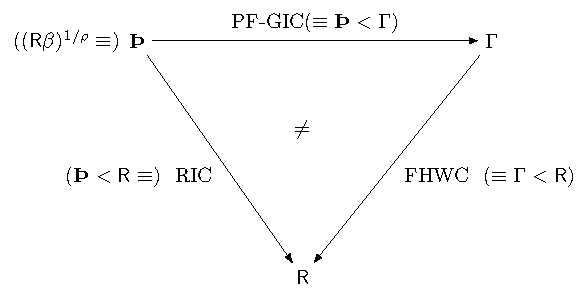
\includegraphics[width=4in]{\FigDir/InequalityPFGICFHWCRIC}
\caption{Inequality Conditions for Perfect Foresight Model \\ (Start at a node and follow arrows)}
\label{fig:InequalityPFGICFHWCRIC}
\end{figure}

\subsection{The Unconstrained Perfect Foresight Model}

A simple illustration of our method is presented in Figure~\ref{fig:InequalityPFGICFHWCRIC}, whose three nodes represent values of the absolute patience factor $\Pat$, the permanent-income growth factor $\PGro$, and the riskfree interest factor ${R}$.  The arrows represent imposition of the labeled inequality condition  (like,  the uppermost arrow, pointing from {$\Pat$} to $\PGro$, reflects imposition of the {\PFGIC} condition (clicking {\PFGIC} should take you to {\PFGICFull}; definitions of other conditions are also linked below).\footnote{For convenience, the equivalent ($\equiv$) mathematical statement of each condition is expressed nearby in parentheses.}  Annotations signified by parenthetical expressions containing $\equiv$ have no content: They are there to make the diagram readable for someone who may not immediately remember terms and definitions from the main text.  (Such a reader might also want to be reminded that ${R}, {\beta}, $ and $\Gamma$ are all in $\mathbb{R}_{+}$ and ${\rho}>1$).

Navigation of the diagram is simple: Start at any node, and deduce a chain of inequalities by following any arrow that exits that node, and any arrows that exit from successive nodes.  Traversal must stop when it reaches a node with no exiting arrows.  So, for example, we can start at the $\Pat$ node and impose the {\PFGIC} and then the {\FHWC}, and conclude that imposition of these conditions allows us to conclude that $\Pat < {R}$.

Negation of a condition is indicated by the reversal of the corresponding arrow.  So, for example, the negation of the {\RIC},  $\cncl{\RIC} \equiv \Pat > {R}$, would be represented by moving the arrowhead from the bottom right to the top left of the line segment connecting {$\Pat$} and ${R}$.

If we were to start at ${R}$ and then impose $\cncl{\FHWC}$, that would reverse the arrow connecting ${R}$ and $\PGro$, but the $\PGro$ node would then have no exiting arrows so no further deductions could be made.  However, if we \textit{also} reversed $\PFGIC$ (that is, if we imposed $\cncl{\PFGIC}$), that would take us to the $\Pat$ node, and we could deduce ${R} > \Pat$.  However, we would have to stop traversing the diagram at this point, because the arrow exiting from the $\Pat$ node points back to our starting point, which (if valid) would lead us to the conclusion that ${R} > {R}$.  Thus, the reversal of the two earlier conditions (imposition of $\cncl{\FHWC}$ and $\cncl{\PFGIC}$) requires us also to reverse the final condition, giving us $\cncl{\RIC}$.  The corresponding algebra is
\begin{equation}\begin{gathered}\begin{aligned}
  \cncl{\FHWC}:~~~~  {R} & < \PGro \notag  
  \\ \cncl{\PFGIC}:~~~~ \PGro & < \Pat %~\left(\equiv ({R} \DiscFac)^{1/{\rho}}\right)
                                \label{eq:cnclRIC}
  \\ \Rightarrow \cncl{\RIC}:~~~~{R} & < \Pat \notag,
\end{aligned}\end{gathered}\end{equation}

% which illustrates another aspect of the diagram: If all arrows are reversed in a partial traversal of the diagram leading to a final step, then the arrow for the final step must also be reversed.  In this case, since both conditions leading to ${R}$ have had their arrows reversed, the arrow coming out of ${R}$ should also be reversed, implying the negation of the {\RIC} -- as \eqref{eq:cnclRIC} proved.

% For clarity, further diagrams will omit multiple arrows indicating reversal of causality (in Figure~\ref{fig:InequalityPFGICFHWCRIC} there would, for example, be only a single arrow, from {$\Pat$} to $\PGro$, at the top level of the diagram).  And definitions of conditions will also be omitted henceforth.

Under these conventions, the main text presents a version of the diagram extended to incorporate the {\PFFVAC} \href{https://econ-ark.github.io/BufferStockTheory/#RelatePFGICFHWCRICPFFVAC}{reproduced in Figure}~\ref{fig:RelatePFGICFHWCRICPFFVAC}).\footnote{For readers familiar with the \href{https://en.wikipedia.org/wiki/Commutative_diagram}{commutative diagrams}, it should be noted that despite the similar appearance, this diagram is not exactly commutative.}%  because the three ways of arriving at the conclusion embodied in the diagonal arrow (the {\PFFVAC}) are NOT identical in their other implications.}

\providecommand{\figName}{RelatePFGICFHWCRICPFFVAC} % Allows generic definition of hypertargets based on title of figure
\providecommand{\figFile}{\figName} %  and on filename
\hypertarget{\figFile-App}{}
\input{\FigDir/\figName} % Read in the tex to generate the figure

This diagram can be interpreted, for example, as saying  that, starting at the $\Pat$ node, it is possible to derive the $\PFFVAC$\footnote{in the form $\Pat < ({R}/\PGro)^{1/{\rho}}\PGro$} by imposing both the {\PFGIC} and the {\FHWC}; or by imposing {\RIC} and \cncl{\FHWC}.  Or, starting at the $\PGro$ node, we can follow the imposition of the {\FHWC} (twice - reversing the arrow labeled $\cncl{\FHWC}$) and then $\cncl{\RIC}$ to reach the conclusion that $\Pat < \PGro$.  Algebraically,
\begin{equation}\begin{gathered}\begin{aligned}
  {\FHWC}:~~~ \PGro & < {R} 
  \\ \cncl{\RIC}:~~~ {R} & < \Pat 
  \\ \PGro & < \Pat \label{eq:cnclPFGIC}
\end{aligned}\end{gathered}\end{equation}
which leads to the negation of both of the conditions leading into $\Pat$.  \cncl{\PFGIC} is obtained directly as the last line in \eqref{eq:cnclPFGIC} and \cncl{\PFFVAC} follows if we start by multipling the Return Patience Factor ({\RPF}=$\Pat/{R}$) by the \FHWF (=$\PGro/{R}$) raised to the power $1/{\rho}-1$, which is negative since we imposed ${\rho} > 1$.  {\FHWC} implies {\FHWF} $< 1$ so when {\FHWF} is raised to a negative power the result is greater than one.
Multiplying the {\RPF} (which exceeds 1 because \cncl{\RIC}) by another number greater than one yields a product that must be greater than one:
\begin{equation}\begin{gathered}\begin{aligned}
  1  & < \overbrace{\left(\frac{({R} \DiscFac)^{1/{\rho}}}{{R}}\right)}^{>1 \text{~from~}\cncl{\RIC}}\overbrace{\left(\PGro/{R}\right)^{1/{\rho}-1}}^{\phantom{...}>1~\text{~from~} \FHWC} \notag
  \\ 1  & < \left(\frac{({R} \DiscFac)^{1/{\rho}}}{({R}/\PGro)^{1/{\rho}}{R}\PGro/{R}}\right) \label{eq:cnclFHWFAndcnclRICImplycnclPFFVAC}
  \\ {R}^{1/{\rho}}\PGro^{1 - 1/{\rho}} = ({R}/\PGro)^{1/{\rho}} \PGro  & < \Pat \notag
\end{aligned}\end{gathered}\end{equation}
which is one way of writing $\cncl{\PFFVAC}$.

The complexity of this algebraic calculation illustrates the usefulness of the diagram, in which one merely needs to follow arrows to reach the same result.

After the warmup of constructing these conditions for the perfect foresight case, we can represent the relationships between all the conditions in both the perfect foresight case and the case with uncertainty as shown in Figure~\ref{fig:Inequalities} in the paper (reproduced below).

\renewcommand{\figName}{Inequalities} % Allows generic definition of hypertargets based on title of figure
\renewcommand{\figFile}{\figName} %  and on filename
\hypertarget{\figFile}{}
\hypertarget{\figName}{}
\input{\FigDir/\figName} % Read in the tex to generate the figure

\begin{CDCPrivate}
  \pagebreak

  % \footnotesize

  For Mateo and Xudong:
  
  I performed all the Google searches I could think of to see if there was an established body of practice for constructing diagrams like the ones we have constructed, but did not find any examples that were particularly close.  

  But the idea of such diagrams is so useful and intuitive that I feel there must be SOME body of practice, that I should be citing (and whose conventions I should be, but may not be, following).

  At first I thought that what we want to do could be done using the conventions of \href{https://mathematica.stackexchange.com/questions/8654/creating-diagrams-for-category-theory}{"category theory diagrams"}. But now I think our diagrams do NOT abide by those conventions, which is why I have labeled them above as ``Relational'' diagrams (and referred to them in the text as ``inequalities diagrams.'')

  My (limited) understanding of category theory from spending a couple of days browsing the web, is that the "nodes" are sets (or some generalization of sets). I had been thinking of the nodes in our diagrams like the simple one in~\ref{fig:InequalityPFGICFHWCRIC} as quantities (numbers).  To see if I could convert the diagrams to category theoretic ones, I have worked out an interpretation in which you can think of the nodes as designating sets.

  My interpretation of our diagrams, however, is one in which the content of a node depends on how you got to it. As best I can understand it, this is NOT the way category theory diagrams work.

  For our diagrams, you can choose the node at which you start, and you can consider the object at that node as containing the set of all potential values of that object. That is, say in the case of $\Pat$, all of the combinations of ${R}$ and ${\beta}$ and ${\rho}$ which satisfy our intrinsic assumptions about those quantities (like ${\rho} > 1$).

So then the interpretation of {\PFGIC} is that it is an operation (``morphism?'') that, for every object in $\Pat$, identifies the subset of values of the $\PGro$ set such that $\Pat$ < $\PGro$ is satisfied. This is a one-to-one mapping: For each real $\Pat$, exactly one (contiguous) set of values of $\PGro$ is identified. Or, if you start at the $\PGro$ node, then the items in that node are all possible values of $\PGro \in (0,\infty)$, and imposition of the FHWC identifies, for each $\PGro_{i}$, the set of values of ${R}$ for which $\PGro < {R}$.

In this example, whether one thinks of the objects in $\PGro$ as values (if you start at $\PGro$) or sets of values indexed by $\Pat$ (e.g., for $\Pat_i$, the content of the node $\PGro$ reached by imposing $\PFGIC$ is the SET of values satisfying $\PGro_{i} $ > $\Pat_i$. This is different from what I have been able to understand about category theory diagrams, in which I believe that the nodes are supposed to contain sets whose content is not "operated upon" but simply mapped by prior operators.

In any case, the diagram is not commutative (if I understand commutativity in this context) in the sense that the set of values of ${R}$ identified by the diagram depends on the route taken to get there.  If we start (and end, because it has no exiting arrows) at the ${R}$ node, its contents should be interpreted as ${R} \in \mathbb{R}_{+}$.  If we start at $\PGro$ and impose {\FHWC}, then the interpretation of the ${R}$ node is, for each $\PGro_{i}$, the set of values of ${R}$ that exceed that $\PGro_{i}$.  If we start at $\Pat$ and impose {\RIC}, when we arrive at ${R}$ it is viewed as containing the set of values that, for each feasible value of $\Pat_{i}$, is greater than that $\Pat_{i}$. And if we start at $\Pat$ and traverse the diagram by first imposing the {\PFGIC} to get to the $\PGro$ node, and then imposing the {\FHWC}, the contents of ${R}$ are doubly indexed. My understanding is that, for the diagram to be commutative, we would need (starting, say, at $\Pat$) for the operations {\RIC} and {\PFGIC} $\circ$ {\FHWC} to be equivalent in their effects on ${R}$. The inequality sign in the center of the diagram is meant to signal the noncomutativity of the paths (a notational convention I found articulated on stackexchange).

Generalizing the point to the next diagram, I have put inequality signs in the upper and lower triangles to signal that the diagram is not commutative. That is, the inequality operators are intended to convey that if you reach the bottommost node by traversing the outside of the diagram (in either direction), that is NOT equivalent to imposing \PFFVAC directly.

Let me emphasize that what we are doing is logically and mathematically sensible under these definitions.  What I'm not sure about is whether

1. The diagram would be misunderstood by a category theorist who would assume that the structure and operations would mean something different than what we want to mean;

2. There is another way to do the diagram that would be equally transparent to non-category-theorists but would satisfy the conventions of category theory.
\end{CDCPrivate}

\onlyinsubfile{\bibliography{\LaTeXFiles/BufferStockTheory,economics}}

\end{document}


% Local Variables:
% eval: (setq TeX-command-list  (assq-delete-all (car (assoc "BibTeX" TeX-command-list)) TeX-command-list))
% eval: (setq TeX-command-list  (assq-delete-all (car (assoc "BibTeX" TeX-command-list)) TeX-command-list))
% eval: (setq TeX-command-list  (assq-delete-all (car (assoc "BibTeX" TeX-command-list)) TeX-command-list))
% eval: (setq TeX-command-list  (assq-delete-all (car (assoc "BibTeX" TeX-command-list)) TeX-command-list))
% eval: (setq TeX-command-list  (assq-delete-all (car (assoc "Biber"  TeX-command-list)) TeX-command-list))
% eval: (add-to-list 'TeX-command-list '("BibTeX" "bibtex ../LaTeX/%s" TeX-run-BibTeX nil t                                                                              :help "Run BibTeX") t)
% eval: (add-to-list 'TeX-command-list '("BibTeX" "bibtex ../LaTeX/%s" TeX-run-BibTeX nil (plain-tex-mode latex-mode doctex-mode ams-tex-mode texinfo-mode context-mode) :help "Run BibTeX") t)
% TeX-PDF-mode: t
% TeX-file-line-error: t
% TeX-debug-warnings: t
% LaTeX-command-style: (("" "%(PDF)%(latex) %(file-line-error) %(extraopts) -output-directory=../LaTeX %S%(PDFout)"))
% TeX-source-correlate-mode: t
% TeX-parse-self: t
% eval: (cond ((string-equal system-type "darwin") (progn (setq TeX-view-program-list '(("Skim" "/Applications/Skim.app/Contents/SharedSupport/displayline -b %n ../LaTeX/%o %b"))))))
% TeX-parse-all-errors: t
% End:
